\documentclass[../root.tex]{subfiles}

\begin{document}

\section{Introduction}
\label{sec:introduction}

Industrial \emph{robots} are programmed to perform highly specialized and
repetitive actions in controlled environments. Therefore, their
autonomy is quite limited and they are restricted to a small set of
problems. We would like that robots that are
not in such controlled scenarios are able solve a larger variety of
problems, and even to react in the presence
of adverse events.
In other words, we
would like robots to reason about their environment and about the
potential effects that their actions may exert on it.
Such capabilities would allow for great flexibility in the following
ways: (1) tasks can be switched without reprogramming; (2) multiple
solutions to the same problem can be found and assessed in terms
of risk and potential gains in execution speed or other criteria; and (3)
contingency mechanisms can be applied, should adverse events hinder
the execution of the task.

We can think of several applications that are potential targets
of these desirable qualities. One possibility is to use robots to assist old and
impaired people for household chores
or treatment~\cite{canal2018adapting,andriella2018deciding}. Another
application is to allow robots to perform maintainance in difficult-to-access
environments, such as subaquatic facilities~\cite{palomeras2016toward,ong2010planning}.

In this document we are concerned with \emph{automatically disassembly}
of electronic devices with a robotic arm. Namely, we want to enable the
robot to retrieve the most valuable and/or dangerous components.
The recycling application is very promising from environmental
and scientific points of view. Our intention is
to provide strategies for performing intelligent action selection.
That is, given a disassembly scenario, the robot should be able
to perform the most suitable action taking into consideration
risk and speed criteria. We tackle this objective using tools
from the area of \emph{Automatic Planning and Scheduling}, namely
probabilistic planning with MDPs (\emph{Markov Decision Processes}).
In this document we explore methods of on-line resolution via
determinization and hierarchical organization of the
identified tasks. We use PPDDL (\emph{Probabilistic Planning Domain
Definition Language}) to define the MDP.

\section{Motivation}

The research presented in this document has been conducted aiming at
developing techniques that can be effectively employed to \emph{recycle}
contraptions such as hard drives, hair trimmers, remote controls or
electronic toys. Fig.~\ref{fig:examples-of-devices} shows some
examples of the devices that we have in mind.

\begin{figure}[tbhp]
	\centering
	\begin{subfigure}[b]{0.31\columnwidth}
		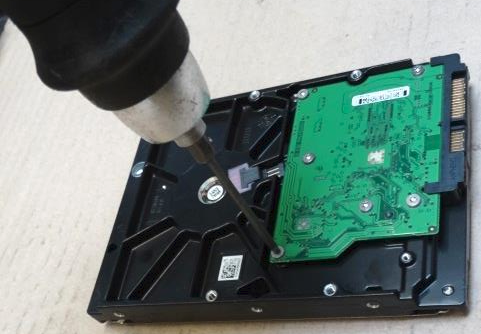
\includegraphics[width=\textwidth]{hddbottom}
		\caption{}
	\end{subfigure}
	~
	\begin{subfigure}[b]{0.31\columnwidth}
		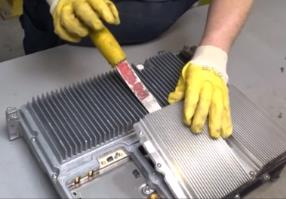
\includegraphics[width=\textwidth]{gsmamp}
		\caption{}
	\end{subfigure}
	~
	\begin{subfigure}[b]{0.31\columnwidth}
		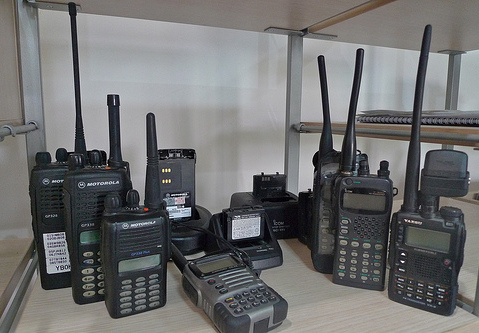
\includegraphics[width=\textwidth]{handies}
		\caption{}
	\end{subfigure}
	\caption{
		(a) Bottom view of a hard drive being disassembled.
		(b) GSM amplifier being disassembled.
		(c) Several handie-talkie models being displayed.
	}
	\label{fig:examples-of-devices}
\end{figure}

In our view, this application poses very attractive challenges
from the scientific point of view. In real life deterministic environments
(i.e. fully observable state variables and non-random action outcomes)
are more an exception than a rule, and this becomes evident in disassembly
scenarios. On the one hand, the whole structure of the device cannot be
perceived at once because of occlusions and perception noise, as
Fig.~\ref{fig:examples-of-devices} illustrates. Therefore, progression
in the disassembly task is required to discover hidden components and
geometrical relations. On the other hand, actions might not produce
always the same outcome, due to positioning errors, noise in the movement
of the robots and exogenous factors. For instance, levering the PCB
of a hard drive in order to extract it from the bay might not success
entirely, leaving the PCB hovering over one of the edges of the casing.
In such case, one may need to consider an additional action like levering
from a different point or holding the case upside down to let the loosen
components fall.

\begin{figure}[tbhp]
	\centering
	\begin{subfigure}[b]{0.45\columnwidth}
		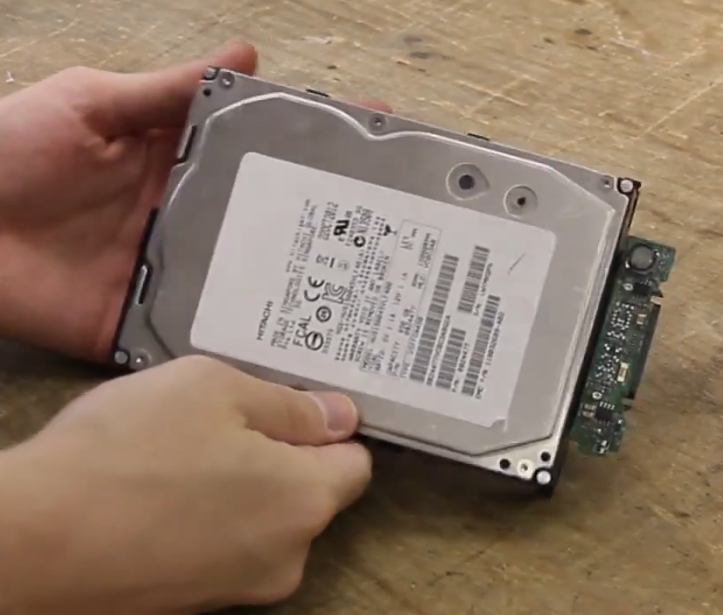
\includegraphics[width=\textwidth]{hddtopcover}
		\caption{}
	\end{subfigure}
	~
	\begin{subfigure}[b]{0.45\columnwidth}
		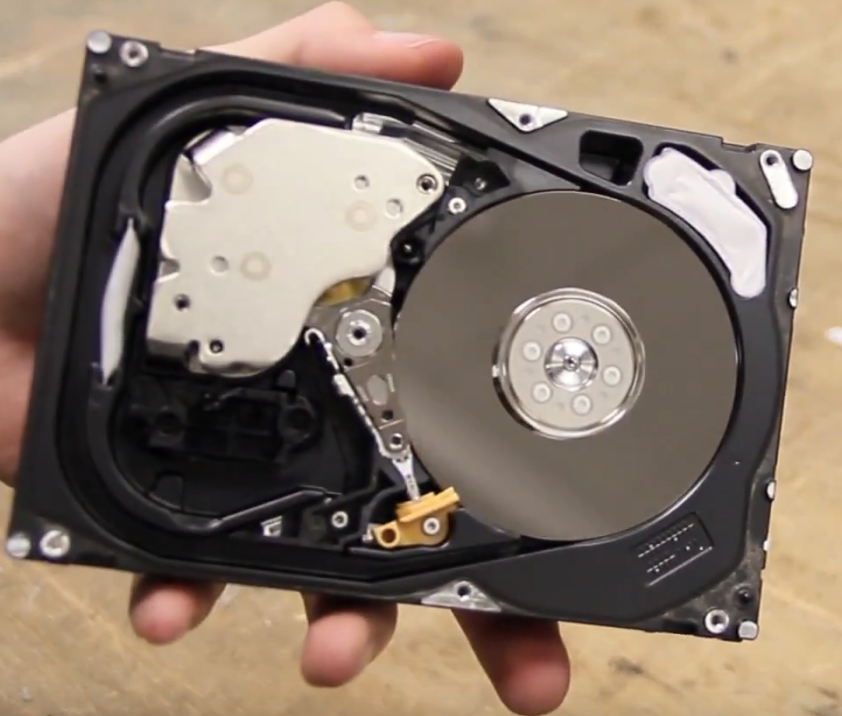
\includegraphics[width=\textwidth]{hddtopwocover}
		\caption{}
	\end{subfigure}
	\caption{
		(a) Top view of a hard drive with the lid.
		(b) View from the same perspective without the lid. The
		previously occluded inner components are now visible.
	}
	\label{fig:example-of-occlusion}
\end{figure}

We cannot forget the social and environmental impact of the
proposed application. The current recycling industry is dominated
by the \emph{crush and separate} paradigm. Trash is crushed into
very small bits that are then filtered and classified using
physical properties such as density or inductance. However,
the uniformity of the separated debris cannot be guaranteed.
Even more importantly, devices often contain components or
substances that are hazardous for the environment. In such cases,
it is required that a human manually removes the source of danger.
This has associated health risks for the operator. Moreover,
it is inefficient and costly, so a great amount of trash is
simply incinerated, posing a serious thread for the ecosystems.
Another drawback of this method is that precious or reusable
components (e.g. PCBs, capacitors, magnets) are destroyed,
when they can be used right away or after some refurnishing
in the manufacturing of new products.

In light of these arguments, a robotic recycling system is
appealing from the sustainability perspective as well.
To avoid the drawbacks of the \emph{crush and separate} method,
we would like the following features for the robot:
(1) it should
ideally adapt to different electromechanical contraptions
(including different brands/models of the same device);
(2) it should correctly identify the tasks that it
has to complete to perform a successful disassembly; and (3)
it should be able to work even with damaged devices.

\section{Involvement in H2020 Imagine}
\label{sec:imagine}

This research has been conducted as part of the European H2020 project
\emph{Imagine: Robots Understanding Their Actions by Imagining Their Effects},
or just \emph{Imagine}\footnote{\url{https://imagine-h2020.eu/}}. The scientific
objective of \emph{Imagine} is to make robots aware of their environment
and, in general, to achieve the autonomy objectives discussed
previously in
Section~\ref{sec:introduction}. The project focuses on the recycling
application introduced in the former section.

There are seven European research centers participating in \emph{Imagine},
each working on a different subsystem. One of these subsystems is a
planning and decision unit, which is developed by the IRI-CSIC 
(\emph{Institut de Rob\`otica i Inform\`atica Industrial}%
\footnote{\url{http://www.iri.upc.edu/}}-%
\emph{Consejo Superior de Investigaciones Cient\'ificas}%
\footnote{\url{http://www.csic.es/}}) partner. This thesis is hosted
in this institution and is closely
related to the development of the \emph{Imagine}'s decision unit.
This subsystem is a fundamental part of the overall system, since it
evaluates the scene and selects the action that is more suitable for
the perceived state. This means that it has to make sure that the action
is beneficial in the long term and that the risk of falling into a
dead end is controlled.

The project also features PHYS and ASC as novel ideas for the considered application.
The first is a very realistic and
powerful physics simulator that can give a very precise idea of the state that results
from executing an action, but makes intensive use of
computational resources. The second is an Association Engine that identifies the
points of interest
of the scene, and also learns a high level physics model (``folks physics'')
that is much quicker to invoke than PHYS, but also less accurate.
They are very useful and have great potential, because the planner can interact
with them and ``imagine'' plans before any action.
Another key aspect of the project is the concept
of ADES, or \emph{Action Description}, for storing the symbolic description
of the actions and the DMPs (\emph{Dynamic Movement Primitive}) associated to
each one. Other aspects of the project include the perception of the scene
and the design and construction of a multifunctional gripper.

\begin{wrapfigure}{L}{0.5\columnwidth}
	\centering
	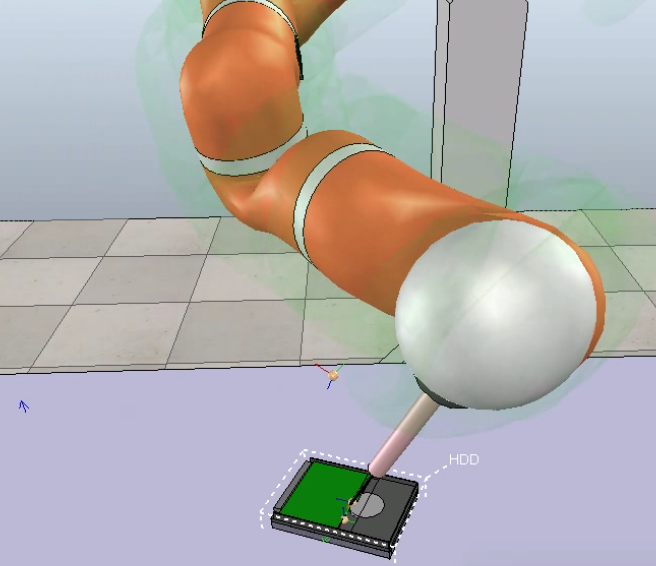
\includegraphics[width=\linewidth]{vrepimage}
	\caption{Execution of a levering action in the V-REP simulator.}
	\label{fig:vrepimage}
\end{wrapfigure}

As of today, we have been participating actively on \emph{Imagine} for more
than a year.
In April of 2018 the project was evaluated by a Project Officer and three experts in
different areas of robotics. It received very positive critics. Part of the
presentation for the evaluation meeting consisted in a demonstration that
displayed basic prototypes of the different subsystems interacting with each
other, and was
able to solve very simple disassembly simulated scenarios
involving a
hard drive (see Fig.~\ref{fig:vrepimage}).
This demonstration already featured a planner prototype in the loop.
Our objectives for this year is to extend this planner with new
capabilities, including the ones presented here, but also with
a rich and beneficial interaction with PHYS and ASC.

\section{Planning concepts}

We see in the area of \emph{Automatic Planning and Scheduling}
tools that potentially bring us toward the
desirable qualities exposed in Section~\ref{sec:introduction}.
Planning is a branch inside Artificial
Intelligence that aims at solving problems that are defined
\emph{declaratively}, with as little control (procedural) knowledge
as possible.
That is, a
planning algorithm
operates with a model that encodes the dynamics of the domain and, for
each problem, outputs
an action sequence
or a policy that solves it, has a high success probability or has a high
expected reward.

Planning is not a discipline that is particular to
robotics and, therefore, there exist multiple benchmarks and work in the
field that is general enough to be of use in many areas. One of the
most successful conferences that spreads knowledge in the field of planning is
ICAPS (International Conference in Automatic Planning and Scheduling)
\footnote{\url{http://www.icaps-conference.org/}}. The conference is
held every year and hosts a competition that seeks to push the boundaries
of the state of the art planning systems.

In this section we seek to give a brief overview of some of the most of
the most important concepts in planning. Later, In Chapter~{chap:theory} we
give a more formal description of the planning language and paradigm that
is relevant for our work.

\subsection{Domain and problem}

One of the common themes in planning is the separation between the \emph{domain}
description and the \emph{problem instance} facts.
This separation is not always present,
since, given a planning paradigm, it is possible to provide an ad-hoc
representation of the problem (e.g. a transitions and reward matrices for an
MDP, or a graph for deterministic problems).
However, the domain/instance concept gives a principled way for defining
problems declaratively
using specialized modeling languages (more on this later).

The domain models the logic of the environment. That is, the predicates
and variables that define the state, and the actions that are available
to the agent(s). This domain is common for all the problems that follow
that share the same logic. For instance, all the problems from the
recycling application would use the same domain, that specifies the
levering and unscrew actions.

On the other hand, each particular instance has associated a set of
facts that are linked to this very problem. That includes the initial state,
the goal condition, the optimization criteria and so on. Let us provide
an example for the recycling scenario: for disassembling a hard drive,
the initial state consists in the specification of the current configuration
of the device, as the robot sees it (the cover and some screws on the top and
the PCB, the motor-PCB connector and some screws on the bottom); the goal
consists in the removal of all the macro-components (the cover and the PCB).
Notice that in this particular example, once the cover is removed, the robot will
be able to see more macro-components and update the goal. The goal can also
include the optimization of some metric (plan length, some measure of cost,
reward...).

\subsection{Planning paradigms}

For our work we focus on goal-based MDPs for representing recycling
problems. However, we think it is illustrative to present the planning
that we have considered in order to justify our choice:

\paragraph{Deterministic planning:} A deterministic planning problem
is given by a graph of states connected by the allowed transitions due
to actions, an initial state and a set
of goal states. Solutions to deterministic problems
consist of ground actions sequences. As the name suggests,
the actions are deterministic (i.e.
they always produce the same outcome), and the state is fully
observable.
PDDL (\emph{Planning Domain Definition Language}~\cite{fox2003pddl2})
is the language of choice for specifying domains and instances in
the \emph{Deterministic Track} of the
IPC (\emph{International Planning Competition}) organized by the
ICAPS. This paradigm is often hard to apply in
the real world because the environments are noisy.
However, in certain applications it is acceptable to assume
that the actions will always render the expected outcomes,
that all the relevant state information is always available and
that small deviations from the expected outcomes are tolerable
and can be handled via replanning. Deterministic planning
has a place within our work, since part of our approach consists
in determinizing a probabilistic domain.

\paragraph{MDP:} MDP stands for \emph{Markov Decision Process}. They
drop the deterministic state-transition assumption and allow for
probabilistic effects. Moreover, MDPs are typically formulated as
reward-maximization problems rather than graph search. However,
we can also think of specific class of MDPs which are goal-based
and that are also also known as SSPPs (\emph{Stochastic Shortest
Path Problem}). In these, there exists a subset of states called
goals or absorbing states. MDPs are specified by the \emph{transition
probability}, the reward function and a discount factor that determines
how important are the long-term versus the short term gains.
The solution for general MDPs are \emph{policies}. That is,
a function that tells the agent which action should it
pick in each state to maximize the accumulated discounted reward
(this is formalized in Chapter~\ref{chap:theory}). The computation of
full or off-line policies is costly in large-scale MDPs,
although there exist on-line methods to overcome this issue.
We apply this paradigm to our problem because it is adequate
for expressing uncertainty about the action outcomes, but stills allows for
efficient solving techniques, avoiding the issues of more sophisticated
techniques. The language
employed in the IPPCs (\emph{International Probabilistic Planning %
Competition}) for describing the domains' logic and the problems'
instances are PPDDL (\emph{Probabilistic PDDL}~\cite{younes2004ppddl1})
and RDDL (\emph{Relational Dynamic Influence Diagram Language}~%
\cite{sanner2010relational}).

\paragraph{POMDP:} POMDPs (\emph{Partially Observable MDP})
introduce an additional level of uncertainty,
dropping the assumption of full observability.
The planning agent no longer has access to the ground truth about the
current state variables. Instead, it receives \emph{observations} that
are drawn from a probability distribution that depends on the true state
and the last executed action. Therefore, the agent operates in belief
space (i.e. a continuous space of probability distributions over all
the possible states). Due to this, the resolution methods
of POMDPs become more sophisticated and intensive from a computational
perspective. While, seemingly, this is the best approach to our
recycling domain, the main source of state uncertainty comes from unknown
objects that cannot be seen due to occlusions. Therefore, the state is
\emph{incomplete} (which is different than unobserved),
and POMDPs would not greatly help at this issue. We assume that other
sources of state
uncertainty can be handled effectively via replanning. The RDDL language
has enough expressivity for specifying POMDPs, too. Other languages
for specifying POMDPs are Cassandra's \texttt{pomdp-sove} file format%
~\cite{cassandra2018pomdp} and PomdpX~\cite{hsu2018pomdpx}.
 
\paragraph{Reinforcement Learning:} Since planning deals
with tuning an agent's
behavior to operate in a certain environment, it is possible to see some
similarities between planning and Reinforcement Learning. The main difference
is that, in their most basic form, a Reinforcement Learning agent is
model-free and dependent on its learning capabilities to decide the
suitable action for a certain state, while a planner takes advantage of a
model of the domain and employs informed search or other heuristic methods to
find a plan (although definitively there
exist works that allow partial domains and that incorporate learning
capabilities to complete them%
~\cite{martinez2017relational,martinez2015vmin}). Reinforcement
Learning is a ``tabula rasa'' framework%
~\cite{sutton2018reinforcement}, while planning takes advantage
of an existing model of the domain to tune the agent's performance.
In Reinforcement Learning it is often assumed (although it is, by no means,
a necessary condition) that the underlying model of the environment follows
the same principles as an MDP, although it is unknown to the agent.

\subsection{Modeling languages}

Above we mentioned a couple of options for modeling MDP
problems in a principled way: PPDDL~\cite{younes2004ppddl1}) and RDDL%
~\cite{sanner2010relational}). These languages allow to easily encode
the dynamics of the environment, and to interpret already encoded
ones. The language of choice for
our work is PPDDL. Here, we give the highlights of both in order
to justify our choice.
Later on, in Chapter~\ref{chap:theory}, we describe PPDDL in more detail.

\paragraph{PPDDL:} effects-based language. That means that
all the transitions are caused by an action executed by the agent(s). All
the possible changes in the state are organized as effects
of the different actions that are available. In fact, PPDDL is just an extension
over PDDL to add probabilistic outcomes to the actions and rewards. PPDDL does not provide any ``iddle'' action nor any language mechanism
for concurrency and exogenous effects (i.e.
effects that are independent of the selected action).
In other words, PPDDL considers that all the changes that may occur in the
state are the result of conscious choices made by the agent.
Much like in PDDL, the state is represented as a collection
of predicates and, optionally and very often with limited support. numeric
state variables. We have chosen PPDDL because an effects-based language
makes it much easier to design and
manipulate the disassembly domain.
The easiness of manipulation becomes specially important for
the determinization techniques.

\paragraph{RDDL:} transition-based language. RDDL regards everything as a
fluent or variable, including the actions and the rewards. The language allows
to specify a transition function for all the state variables. The transition
function may depend on the executed action and the previous state variables'
values. It can be defined stochastically as well. Therefore, RDDL has
the potential of expressing domain logics
with exogenous effects much more naturally than PPDDL. However, since the
changes are not grouped into action, some domains that can be written very
easily in PPDDL are somewhat more tedious to reproduce in RDDL. The main
reason we have chosen PPDDL over RDDL, however, is that RDDL makes it
considerably harder to implement the determinization techniques that we
explore in this document. Since we do not need the additional expressivity
of RDDL, this is not a big concern. As a side note, RDDL is expressive
enough to also represent partial observability.

\section{Approach}

As said before, we resort to the MDP
formalism to express our problem, capturing the uncertainty over
the state transitions.
One of the main limitations of MDPs for
real-life problems is that they assume full observability of the state variables.
In practice, this is not true for our application. However, dropping this
assumption results in POMDPs, whose resolution is computationally costly
and scales badly with the size of the state space. Moreover, POMDPs do
not provide any substantial expressivity gain when the agent does not know all
the state variable, which happens when the agent is not aware of all
the relevant objects of the scene.

We update and solve a new MDP each
time the specification of the state changes (i.e. when new objects are discovered
after performing an action).
Even though solving MDPs is much less intensive than
solving POMDPs, conventional algorithms that obtain a full policy, such
as \emph{Value Iteration} and
\emph{Policy Iteration}, still suffer from the curse of dimensionality when there
are many state variables due to the \emph{curse of dimensionality}.
Then, computing a full policy becomes infeasible.
We explore two complementary strategies for dealing with this: (1)
determinization algorithms together with classical planners; and (2)
decompositon of the main goal into sub-goals, taking advantage of the
topological precedences imposed by some geometrical
and physical features (e.g. partial occlusion).

The first of these two strategies consists in constructing a deterministic
version of the problem and solving the determinized problem with a planner
such as Fast Forward\footnote{%
\url{https://fai.cs.uni-saarland.de/hoffmann/ff.html}}~\cite{hoffman2001ff} or
Fast Downward\footnote{\url{http://www.fast-downward.org/}}~\cite{helmert2006fast}.
The rationale behind this idea is that solving the determinized problem
is typically much faster than computing an off-line policy. The first
action suggested by the deterministic planner is executed and then the process
is repeated for the next state. Optionally, we can cache plans to
execute them in sequence if everything goes according to expectation (i.e.
the agent does not replan until a deviation from the expected outcomes is
detected).
Good determinization strategies encode the stochasticity of the outcomes
somehow (e.g. as action costs), so the classical planner comes up with plans
that make sense from the probabilistic perspective or, in other words, have
a good chance of succeeding.

The second strategy has more to do with limiting the planning complexity.
The recycling domain is a good candidate for task decomposition, since
there are clear precedence relations between components. For instance,
it makes sense to disassemble the R/W arm of a hard drive before the
platters, because the arm may move and block the platters. The robot
can identify the macro-components that are worth retrieving as the main
tasks, and sort them topologically given the precedence relations. Then,
the planner solves one small task at a time, without caring about
the rest and omitting from the state the facts and variables that are not
relevant for the selected task.

\section{Scope and goals}

The present work revolves mainly around probabilistic planning, without focusing too much
on topics such as scene perception and low-level robot control.
We present tools for modeling stochastic problems from the recycling
domain, as well as techniques for
dealing efficiently with these problems. Although all the examples and benchmarks
have been conceived for the particular use case of the hard drive,
the techniques described here can be extrapolated to other devices by extending
the state specification with variables particular to these devices.

More specifically we:
\begin{itemize}
	\item propose a set of predicates to represent the different components of
	the device and their relation to other components. These are used to represent
	the world state.
	\item propose a PPDDL (\emph{Probabilistic Planning Domain Definition Language})
	model for the recycling domain. This model contains the schemata of the actions
	that can be applied in the domain, as well as the specification of the
	state variables (predicates and functions). PPDDL defines an action-based
	DBN (\emph{Dynamic Bayes Network}) with full observability or, equivalently,
	a MDP.
	\item explore and test several determinization techniques to achieve fast
	approximate on-line solutions to MDPs. The rationale is to avoid costly policy
	recalculations each time the state specification changes when new objects
	are discovered (e.g. after removing the lid of a hard drive). The considered
	determinization algorithms are: (1) All-Outcome and Single-Outcome;
	(2) Alpha-Cost Transition Likelihood; (3) Hindsight optimization.
	\item complement the previous technique with hierarchical planning, taking
	advantage of the strong precedences that arise naturally in the
	considered application. This occurs, for instance, when the read
\end{itemize}

We assess the effectiveness of these strategies testing them against
benchmark problems. On the one hand, we have all the problems from past
IPPCs
(\emph{International Probabilistic Planning Competitions}, hosted
each year by the ICAPS). These are useful to evaluate the suitability of
the different
determinization strategies in domains different from ours. On the other hand,
we have hand-crafted a set of benchmark problems that consist of
hard drive variations with different disposition of components. The determinization
algorithms are evaluated on top of these, too. In addition, these serve
the purpose of assessing the computational gain of the hierarchical planning
method that is specific for the recycling domain.

\section{Related work}

In this section we review some contributions that are related
somehow to our own work. Some of these contributions are purely
theoretical, while others are practical recycling stations.

\begin{wrapfigure}{R}{0.4\columnwidth}
	\centering
	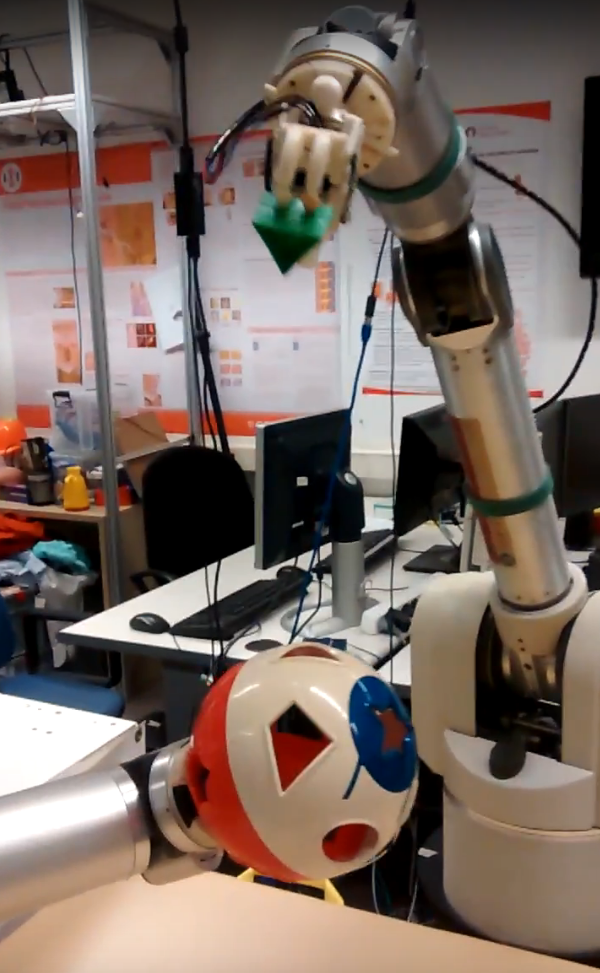
\includegraphics[width=\linewidth]{wamsphere}
	\caption{Barrett WAM robotic arm inserting a triangular piece through
		a cavity with the same shape}
	\label{fig:wamsphere}
\end{wrapfigure}

G-Pack~\cite{kolobov2012blrtdp} and PROST~\cite{keller2013atrial}
are two state-of-the art probabilistic
planners that operate with RDDL (Gourmand actually operates with a PPDDL dialect
that results from translating RDDL models) and provide on-line solutions to
the input MDPs. They interact with a server that sends the most recent state.
They have outperformed the rest of the planners of the 2011
and the 2014
IPPC. Gourmand is based on the \emph{Labeled Real-Time Dynamic Programming}
algorithm~\cite{bonet2003labeled}, while PROST uses \emph{Monte Carlo Tree-Search}
with the UCT (\emph{Upper Confidence bound applied to Trees}) variant%
~\cite{kocsis2006bandit}. Both
algorithms perform well in an on-line setting, with no one being consistently
better than the other in all the IPPC benchmarks, and are worth of consideration
in future work.

Our previous work~\cite{suarez2018interleaving} is
also relevant. We illustrate how to apply concepts of hierarchical and
probabilistic planning to a manipulation task that is comparable with an
assembly scenario (the inverse of the problem covered in this document),
as shown in Fig.~\ref{fig:wamsphere}. Much like in the present work,
geometrical concerns play an important role in the planning task.

The work of Kaelbling and Lozano-Pérez~%
\cite{kaelbling2011hierarchical} deals with hierarchical planning in
a way that is very similar to our approach. In a more recent paper%
~\cite{kaelbling2013integrated} they combine this hierarchical planning
approach with probabilistic planning in belief space. Very much like us,
they base their resolution method in determinizing the SSPP that results
from their formulation. The determinization they propose is called
Alpha-Cost Transition Likelihood. This is one of the methods we employ in our
own research. 

On a more practical level, a recent robotic systems that is more
closely related to the application
presented here is \emph{Liam} (showed in Fig.~\ref{fig:liam}), developed by Apple~\cite{kamps2016apple}.
Liam is a recycling robot specially conceived to dismantle \emph{iPhone}
devices. It is equipped with tools for rescuing the most critical components:
the battery, the camera and the logic board. While the details of the robot
are not revealed, it would seem that it has been designed for operating
in highly controlled environments and following a scripted sequence of
actions for retrieving and classifying the different components. In other
word, the system is tuned to work with a single type of device, while our
goal is to work toward a more general recycling robot.

\begin{wrapfigure}{L}{0.5\columnwidth}
	\centering
	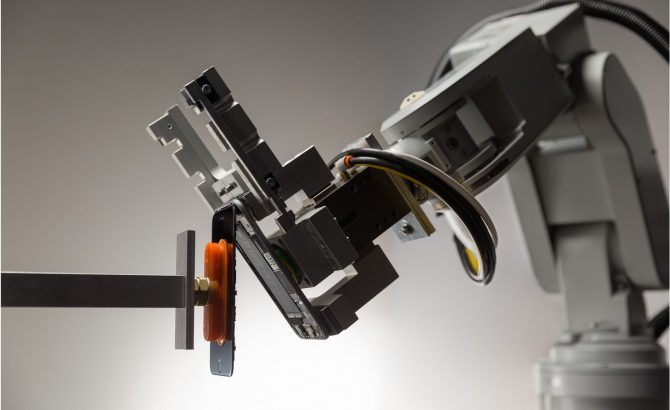
\includegraphics[width=\linewidth]{liam}
	\caption{Liam robot removing the screen of an iPhone device.
		Source: \url{https://youtu.be/AYshVbcEmUc}}
	\label{fig:liam}
\end{wrapfigure}

The work of Torres \textit{et al}~\cite{torresa2003disassembly} falls
directly within the recycling application. In fact, it belongs to the
Spanish CICYT project (\emph{Sistema Robotizado de Desensamblado
Automático basado en Modelos y Visión Artificia}). Much like us, they
seek find disassembly sequences for an electromechanical device. They
represent these devices as graphs and automatically detect clusters of
components and topological dependencies. However, they do not consider
stochasticity.

Finally, it is also worth considering the paper of
Zhang \textit{et al} on part removal~\cite{zhang2008dplan}. They propose
a method for removing parts from a device with collision free paths. It
is more concerned than us with the physical aspects of the problem,
rather than with complex long-term goals and interdependences between
components. In the future, we would like to incorporate some degree
of low-level information into the planner within the Imagine project.
PHYS and ASC, presented in Section~\ref{sec:imagine}, are invaluable
tool to do this.

\IfEq{\jobname}{\detokenize{root}}{}{\printbibliography}

\end{document}